\graphicspath{{chapters/gradient_descent/}}


\chapter{Efficient Algorithms for the CCA Family: Unconstrained Losses with Unbiased Gradients}\label{ch:gradient_descent}
\epigraph{It seems easier to train a bi-directional LSTM with attention than to compute the SVD of a large matrix}{Chris Ré}\citep{gemp2021}
\minitoc
% chktex-file 44
% chktex-file 3
\section*{Preface}
The content of this chapter is based on a series of papers~\citep{chapman2022generalized, chapman2023efficient} as well as a NeurIPS workshop paper~\citep{chapman2023cca}.
I am grateful to my co-authors Lennie Wells and Ana Lawry Aguila for their contributions to this work.
In particular, Lennie's mathematical expertise improved the theoretical grounding of the idea greatly and Ana's access to the UK Biobank dataset enabled the application of our methods to a real-world biomedical dataset.
In this thesis I include much of the work from these papers, but I exclude many of Lennie's extensive proofs where I can make no claim to have contributed beyond proofreading.

Here's an improved introduction that addresses the points you mentioned:
\section{Introduction}
Generalized Eigenvalue Problems (GEPs) are fundamental to a wide range of machine learning algorithms, including Canonical Correlation Analysis (CCA), Partial Least Squares (PLS), Principal Component Analysis (PCA), Independent Component Analysis (ICA), and Linear Discriminant Analysis (LDA). Solving high-dimensional GEPs is a critical challenge in many applications, as classical algorithms often struggle with the computational complexity and numerical instability that arise when dealing with large-scale datasets. This has motivated the development of stochastic algorithms that aim to approximate the solutions of GEPs in a more efficient and scalable manner.
Stochastic algorithms for simple Eigenvalue Problems (EPs), where the matrix $B$ in the GEP is the identity matrix, have been extensively studied and have shown promising results \citep{arora2012stochastic,arora2016stochastic}. These algorithms not only offer computational advantages but also introduce a form of implicit regularization through the noise in the stochastic updates, which can be particularly beneficial in high-dimensional settings. The regularizing effect of stochastic algorithms has been shown to improve generalization performance and robustness to noise, making them an attractive alternative to batch learning algorithms.
However, when it comes to solving more complex GEPs, such as those arising in CCA and PLS, the existing stochastic algorithms have some limitations that hinder their practical applicability. For instance, the $\gamma$-EigenGame algorithm \citep{gemp20,gemp2021} requires the tuning of a hyperparameter $\gamma$ that controls the trade-off between computational efficiency and the accuracy of the stochastic updates. Finding the optimal value of this hyperparameter can be challenging and may vary depending on the problem and the data, making the algorithm less convenient to use in practice.
Another limitation is that some stochastic algorithms, like the Stochastic Generalized Hebbian Algorithm (SGHA) \citep{chen2019constrained}, rely on heuristic primal-dual update rules rather than a principled optimization framework. This makes it difficult to integrate these algorithms with more sophisticated optimizers like Adam \citep{kingma2014adam}, which have been shown to improve convergence speed and stability in many machine learning applications.
To address these limitations and provide a more principled and robust approach to solving GEPs in the stochastic setting, we propose a novel formulation of the CCA problem based on the Eckhart--Young--Minsky inequality \citep{stewart_matrix_1990}. Our formulation leads to a new objective function that characterizes the top-$K$ subspace of GEPs, including CCA as a special case. Importantly, this objective function is unconstrained and can be optimized using standard stochastic gradient descent or batch gradient descent methods, making it compatible with modern optimization techniques.
The key advantages of our proposed approach are:
\begin{itemize}
    \item It provides a unified framework for solving a wide range of GEPs using a single unconstrained objective function, making it applicable to CCA, PLS, PCA, ICA, LDA, and other problems that can be formulated as GEPs.
    \item The objective function can be efficiently optimized using stochastic gradient descent or batch gradient descent, allowing for seamless integration with state-of-the-art optimizers like Adam.
    \item The stochastic nature of the optimization introduces implicit regularization, which can improve the generalization performance and robustness of the learned subspaces.
    \item The approach is more principled and theoretically grounded compared to heuristic primal-dual update rules used in some existing stochastic algorithms.
\end{itemize}

In the following sections, we will provide a detailed background on GEPs and their applications in subspace learning, discuss the limitations of existing stochastic algorithms, and present our novel formulation and optimization approach. We will also demonstrate the effectiveness of our method through extensive empirical evaluations on various datasets and compare its performance with state-of-the-art stochastic CCA and PLS algorithms.

\section{Background: Efficient Solutions to GEPs}\label{sec:background-unified}
\subsection{Solving High-Dimensional Generalized Eigenvalue Problems}
Generalized Eigenvalue Problems (GEPs) play a crucial role in many machine learning algorithms, including Canonical Correlation Analysis (CCA), Partial Least Squares (PLS), Principal Component Analysis (PCA), Independent Component Analysis (ICA), and Linear Discriminant Analysis (LDA). A GEP is defined by two matrices $A$ and $B$, where the goal is to find a vector $u$ and a scalar $\lambda$ that satisfy the equation:
\begin{equation}
Au = \lambda Bu
\end{equation}
The vector $u$ is called the generalized eigenvector, and the scalar $\lambda$ is called the generalized eigenvalue. In the special case where $B$ is the identity matrix, the GEP reduces to a standard Eigenvalue Problem (EP).
Solving GEPs becomes challenging when dealing with high-dimensional data, where the matrices $A$ and $B$ can be very large. The computational complexity of classical algorithms for solving GEPs, such as the power method, scales cubically with the size of the matrices, making them infeasible for large-scale problems. Moreover, when the matrices are ill-conditioned or nearly singular, these algorithms can suffer from numerical instability, leading to inaccurate or unreliable solutions.

\subsection{Unified GEP formulation for CCA, Ridge CCA, PLS, and PCA}
As discussed in \ref{ch:background}\ref{sec:classical-subspace-learning-algorithms}, CCA, ridge-regularized CCA, PLS, and even PCA can be formulated as GEPs with specific structures. This unified formulation involves block matrices $A$ and $B_\alpha$ defined as:
\begin{align}
A^{(ij)} &= \Cov(X\sps{i}, X\sps{j}) \text{ for } i \neq j, \
B_\alpha^{(ii)} &= \alpha_i I_{D\sps{i}} + (1-\alpha_i) \Var(X\sps{i}),
\end{align}
where $\alpha \in [0,1]^I$ is a vector of ridge penalty parameters, $X\sps{i}$ represents the $i$-th view of the data, and $D\sps{i}$ is the dimensionality of the $i$-th view.
By adjusting the values of $\alpha$, we can recover various subspace learning methods:

Pure CCA: Setting $\alpha_i = 0 : \forall i$ recovers the classic CCA problem.
Ridge Extensions: Smoothly transitioning to ridge-regularized CCA or PLS by selectively adjusting values within $\alpha$.
PCA Subsumption: PCA emerges as a single-view form of ridge-regularized PLS.

This unified formulation allows us to focus on solving the core CCA problem, with the understanding that the insights and solutions developed will naturally generalize to the entire family of methods and GEPs more generally.

\subsection{Classical Methods for Solving CCA}
\subsubsection{Eigendecomposition-based Solution}
One common technique to solve the GEP for CCA is to transform it into a standard eigenvalue problem:
\begin{equation}
B^{-\frac{1}{2}} A B^{-\frac{1}{2}} y = \lambda y
\end{equation}
followed by eigendecomposition. This approach is based on the observation that if $(u, \lambda)$ is a generalized eigenpair of $(A, B)$, then $(B^{-\frac{1}{2}}u, \lambda)$ is an eigenpair of $B^{-\frac{1}{2}} A B^{-\frac{1}{2}}$.
An alternative approach is to solve the eigenvalue problem:
\begin{equation}
B^{-1} A v = \lambda v
\end{equation}
However, this approach requires computing the inverse of $B$, which can be numerically unstable and computationally expensive, especially when $B$ is ill-conditioned or nearly singular. In contrast, the $B^{-\frac{1}{2}} A B^{-\frac{1}{2}}$ formulation only requires computing the square root of $B$, which can be done more efficiently and stably using techniques like the Cholesky decomposition.
Nonetheless, both approaches have a computational complexity of $\mathcal{O}((p_1+p_2)^3)$ and may suffer from numerical instability, especially when $B$ is ill-conditioned or nearly singular.

\subsubsection{Classical Iterative Algorithms}
Classical iterative algorithms, such as the power method, Sanger's rule (Generalized Hebbian Algorithm), and Oja's rule, can be used to solve the GEP for CCA. These algorithms are based on the idea of iteratively updating the eigenvector estimates using matrix-vector multiplications.
The power method is a simple iterative algorithm for finding the dominant eigenvector of a matrix $A$. The update rule for the power method is:
\begin{align}
u \leftarrow \frac{A u}{|A u|}
\end{align}
where $u$ is the current estimate of the dominant eigenvector. The power method converges to the dominant eigenvector of $A$ under mild conditions.
Sanger's rule, also known as the Generalized Hebbian Algorithm (GHA), is an iterative learning rule for finding the principal components of a data set. It can be written as:
\begin{align}
U \leftarrow U + \eta \left( A U - U \text{tril}(U^T A U) \right)
\end{align}
where $\text{tril}(\cdot)$ denotes the lower triangular part of a matrix.
Oja's rule, a simplified version of Sanger's rule, can be written as:
\begin{align}
U \leftarrow U + \eta \left( A U - U (U^T A U) \right)
\end{align}
To maintain orthogonality of the eigenvectors during the iterative updates, Oja's rule can be combined with a QR decomposition step:
\begin{align}
U \leftarrow U + \eta \left( A U - U (U^T A U) \right) \
U \leftarrow \text{qr}(U)
\end{align}
where $\text{qr}(\cdot)$ denotes the QR decomposition, which factorizes a matrix into an orthogonal matrix $Q$ and an upper triangular matrix $R$. By using only the orthogonal matrix $Q$, we ensure that the eigenvectors remain orthogonal throughout the iterative process. Alternatively, other orthogonalization techniques such as the Gram-Schmidt process can be employed.
These iterative algorithms can be extended to solve the generalized eigenvalue problem $A U = B U \Lambda$, where $B$ is a positive definite matrix. The update rule for this problem is:
\begin{align}
U \leftarrow U + \eta \left( A U - B U \text{tril}(U^T A U) \right)
\end{align}
which subsumes the original GHA as a special case when $B=I$.
While these classical iterative algorithms can be computationally efficient, especially for sparse or structured matrices, they may suffer from slow convergence and sensitivity to initialization.

\subsubsection{PCA-CCA}
To reduce the computational complexity of solving the GEP for CCA, the PCA-CCA method first applies PCA to each view of the data separately and then solves the GEP in the reduced space. This approach has two main steps:

\begin{itemize}
    \item Apply PCA to each view: Compute the top $K_1$ and $K_2$ principal components for each view, with complexity $\mathcal{O}(p_1^3 + p_2^3)$.
    \item Solve the GEP in the reduced space: Solve the GEP in the reduced space of size $(K_1 + K_2) \times (K_1 + K_2)$, with complexity $\mathcal{O}((K_1 + K_2)^3)$.
\end{itemize}

The overall complexity of PCA-CCA is thus $\mathcal{O}(p_1^3 + p_2^3 + (K_1 + K_2)^3)$, which can be significantly lower than the direct solution when $K_1 \ll p_1$ and $K_2 \ll p_2$.
However, it's important to note that even the PCA step can be computationally expensive for high-dimensional data. In the case where the number of samples $n$ is smaller than the dimensionalities $p_1$ and $p_2$, the maximum number of principal components is $K_1 = K_2 = n$. The complexity of PCA in this case is $\mathcal{O}(n^3 + n^3)$, and the overall complexity of PCA-CCA becomes $\mathcal{O}(2n^3 + (2n)^3) = \mathcal{O}(10n^3)$. While this is lower than the direct solution, it can still be prohibitive for large sample sizes.
\subsubsection{Kernel CCA}
Kernel CCA (KCCA) is another approach that offers computational advantages for high-dimensional data. KCCA maps the original data to a high-dimensional feature space using a kernel function and then performs CCA in that space. The main advantage of KCCA is that its complexity scales with the number of samples $n$ rather than the dimensionalities $p_1$ and $p_2$.
The optimization problem for KCCA can be written as:
\begin{align}
& \alpha_{\text{opt}} = \underset{\alpha}{\mathrm{argmax}} { \alpha\sps{1} K\spsT{1} K\sps{2} \alpha\sps{2} } \
& \text{subject to:} \notag \
& \alpha\sps{1} K\spsT{1} K\sps{1} \alpha\sps{1} = 1 \notag \\
& \alpha\sps{2} K\spsT{2} K\sps{2} \alpha\sps{2} = 1 \notag
\end{align}
where $\alpha\sps{i}$ are dual variables, $K\sps{i}$ are kernel matrices defined as $K\sps{i} = \phi(X\sps{i})\phi(X\sps{i})^T$, and $\phi(\cdot)$ is a nonlinear mapping function.
The complexity of KCCA is $\mathcal{O}(n^3)$, which can be much lower than the direct solution when $p_i > n$. However, KCCA has some significant drawbacks:
\begin{itemize}
    \item The need to store and manipulate the kernel matrices, which have size $n \times n$. This can be memory-intensive for large sample sizes.
    \item The requirement to access all training data at test time, which raises concerns about efficiency and scalability.
    \item The difficulty in interpreting the results in the original feature space, as the learned projections are in the high-dimensional kernel space.
\end{itemize}

In summary, classical methods for solving CCA, such as eigendecomposition-based solutions, iterative algorithms, PCA-CCA, and KCCA, offer various trade-offs between computational complexity, numerical stability, and interpretability. However, these methods may still be prohibitively expensive for high-dimensional data, motivating the development of stochastic algorithms that can efficiently approximate the solution of the CCA problem.

\subsection{Stochastic Algorithms for CCA}
Stochastic algorithms have gained popularity as an alternative approach to solving large-scale CCA problems. These algorithms aim to approximate the solution of the CCA problem by processing the data in small batches or even one sample at a time, making them more efficient and scalable than batch methods.
The key idea behind stochastic algorithms is to update the estimates of the canonical variables incrementally as new data arrives, rather than waiting for the entire dataset to be available. This incremental update scheme allows stochastic algorithms to scale to large datasets and handle data that may not fit into memory.
However, a major challenge in stochastic GEPs and stochastic CCA is the data-dependent constraint $U^\top B U = I$, where the matrix $B$ is unknown and is an expectation of random estimates. In the population setting, $B$ is defined as:
\begin{equation}
B = \begin{pmatrix}
\Sigma_{11} & 0 \\
0 & \Sigma_{22}
\end{pmatrix}
\end{equation}
where $\Sigma_{11} = \mathbb{E}[X^{(1)^\top} X^{(1)}]$ and $\Sigma_{22} = \mathbb{E}[X^{(2)^\top} X^{(2)}]$ are the population covariance matrices of the two views.
In practice, we only have access to sample estimates of these covariance matrices, which introduces additional noise and estimation error. Stochastic algorithms must account for this uncertainty and adapt their update rules accordingly.

\subsubsection{Stochastic Power Method for PLS}
\citet{arora2016stochastic} demonstrate that PLS can be approximated by applying a stochastic power method. The stochastic power method is a simple iterative algorithm that updates the estimates of the left and right singular vectors $U^{(1)}$ and $U^{(2)}$ using the following rules:
\begin{align*}
U^{(1)}_t &= \mathcal{P}_{\text{orth}} \left( U^{(1)}_{t-1} + \eta_t X_t^{(1)} (X_t^{(2)})^\top U^{(2)}_{t-1} \right), \\
U^{(2)}_t &= \mathcal{P}_{\text{orth}} \left( U^{(2)}_{t-1} + \eta_t X_t^{(2)} (X_t^{(1)})^\top U^{(1)}_{t-1} \right),
\end{align*}
where $\mathcal{P}_{\text{orth}}(\cdot)$ represents an orthogonal projection operator that projects a vector or matrix onto the space orthogonal to the current subspace, $X_t^{(1)}$ and $X_t^{(2)}$ are the new data points at time $t$, and $\eta_t$ is the learning rate.
Intuitively, the update rule for $U^{(1)}_t$ can be understood as follows:

The term $X_t^{(1)} (X_t^{(2)})^\top U^{(2)}_{t-1}$ computes the correlation between the new data point $X_t^{(1)}$ and the current estimate of the right singular vector $U^{(2)}_{t-1}$, weighted by the corresponding $X_t^{(2)}$.
This correlation term is then added to the current estimate of the left singular vector $U^{(1)}_{t-1}$, effectively updating it in the direction that maximizes the covariance between the views.
The orthogonal projection operator $\mathcal{P}_{\text{orth}}(\cdot)$ ensures that the updated estimate remains orthogonal to the previous estimates, preventing the algorithm from converging to a suboptimal solution.

The update rule for $U^{(2)}_t$ follows a similar logic, with the roles of $X_t^{(1)}$ and $X_t^{(2)}$ reversed.

The stochastic power method has a low computational complexity of $\mathcal{O}(k(p_1+ p_2))$ per iteration, where $k$ is the number of components being estimated. However, it has some limitations:

Convergence is not guaranteed, as the algorithm may oscillate or diverge in some cases.
The orthogonal projection step does not extend naturally to the CCA problem, where the constraints involve the matrix $B$ (i.e., $U^\top B U = I$) rather than the identity matrix (i.e., $U^\top U = I$).

Despite these limitations, the stochastic power method provides valuable insights into the design of stochastic algorithms for CCA and serves as a foundation for more advanced methods.
\subsubsection{Stochastic Generalized Hebbian Algorithm (SGHA)}
The Stochastic Generalized Hebbian Algorithm (SGHA), proposed by \citet{chen2019constrained}, is an extension of the Generalized Hebbian Algorithm (GHA) to the stochastic setting. SGHA aims to find the top-$k$ generalized eigenvectors of a matrix pair $(A, B)$, where $A$ is symmetric and $B$ is symmetric positive definite.
SGHA formulates the constrained optimization problem for the top-$k$ subspace as:
\begin{align}
\min_{U} -\Tr \left(U^T A U\right) \quad \text{subject to} \quad U^T B U = I
\end{align}
Using Lagrange multipliers, this constrained problem can be transformed into an unconstrained one:
\begin{align}
\min_{U} -\Tr\left(U^T A U \right) + \lambda \left(U^T B U - I\right)
\end{align}
Differentiating with respect to $U$ and $\lambda$ and setting the derivatives to zero yields the stationary points:
\begin{align}
2 A U - 2 B U \lambda = 0 \quad \text{and} \quad U^T B U - I = 0 \
\implies \lambda = U^T A U
\end{align}
Based on these stationary points, SGHA proposes a primal-dual update rule:
\begin{align}
U \leftarrow U - \eta \left( A U - B U \lambda \right) \
\lambda \leftarrow \left( U^T A U \right)
\end{align}
where $\eta$ is a learning rate.
These updates can be combined into a single update rule:
\begin{align}
U \leftarrow U - \eta \left( A U - B U \left( U^T A U \right) \right)
\end{align}
Intuitively, the SGHA update rule can be understood as follows:

The term $A U$ computes the correlation between the current estimate of the generalized eigenvectors $U$ and the data matrix $A$.
The term $B U \left( U^T A U \right)$ serves as a correction term that ensures the orthogonality of the eigenvectors with respect to the matrix $B$. The matrix $\left( U^T A U \right)$ can be interpreted as an estimate of the generalized eigenvalues.
The difference between these two terms is then used to update the current estimate of the eigenvectors $U$ in the direction that maximizes the objective function.

SGHA has a computational complexity of $\mathcal{O}(k^2(p_1+ p_2))$ per iteration, which is higher than that of the stochastic power method but still much lower than the batch methods.
While SGHA is simple to implement, it relies on a heuristic primal-dual update rule rather than a principled optimization framework. This makes it difficult to integrate with more sophisticated optimizers like Adam \citep{kingma2014adam}, which have been shown to improve convergence speed and stability in many machine learning applications.
\subsubsection{$\gamma$-EigenGame for CCA}
The $\gamma$-EigenGame, proposed by \citet{gemp20,gemp2021}, is a stochastic algorithm for CCA inspired by the EigenGame algorithm for PCA. The key idea behind the $\gamma$-EigenGame is to view the generalized eigenvectors as competing players in a game, where each player tries to maximize its own utility function.
In this game-theoretic formulation, the utility function of each player (eigenvector) $u_i$ consists of a reward term and a penalty term:
\begin{align}
\max_{u_i} \overbrace{\frac{u_i^TAu_i}{u_i^TBu_i}}^{\text{reward}} - \overbrace{\sum_{j < i} \frac{(u_j^TAu_j)(u_i^TBu_j)^2}{(u_j^TBu_j)^2(u_i^TBu_i)}}^{\text{penalty}}
\end{align}
The reward term $\frac{u_i^TAu_i}{u_i^TBu_i}$ encourages the eigenvector $u_i$ to align with the direction of maximum correlation between the views, while the penalty term $\sum_{j < i} \frac{(u_j^TAu_j)(u_i^TBu_j)^2}{(u_j^TBu_j)^2(u_i^TBu_i)}$ discourages $u_i$ from aligning with the directions already captured by the previous eigenvectors $u_j$ for $j < i$.
The $\gamma$-EigenGame proposes an update rule for each eigenvector $u_i$ based on this utility function. In the stochastic setting, the algorithm introduces an additional hyperparameter $\gamma$ that controls the trade-off between computational efficiency and the accuracy of the stochastic updates. The update rule is modified to use a rolling average of the matrix $B$, which helps to reduce the computational complexity and memory requirements of the algorithm.
While the $\gamma$-EigenGame has shown promising results in practice, it still requires the tuning of both the hyperparameter $\gamma$ and a learning rate, which can be challenging and may depend on the specific problem and data at hand.
Moreover, the use of a rolling average of the matrix $B$ introduces additional approximation error and may not fully capture the uncertainty in the stochastic orthogonality constraint $U^\top B U = I$.

\subsubsection{Benefits and Limitations of Stochastic Algorithms}
Stochastic algorithms offer several benefits over batch methods for solving CCA problems, such as computational efficiency, implicit regularization, and online learning capabilities. However, they also have some limitations, particularly in the context of stochastic GEPs and stochastic CCA:

Convergence: The convergence of stochastic algorithms can be slower than batch methods, especially in the presence of noise or when the data is highly correlated. The choice of learning rate and mini-batch size can have a significant impact on the convergence speed and stability.
Hyperparameter tuning: Most stochastic algorithms require the tuning of several hyperparameters, such as the learning rate, mini-batch size, and regularization parameters. The optimal values of these hyperparameters can vary depending on the problem and the data, making it challenging to achieve consistent performance across different datasets.
Stochastic orthogonality constraint: The data-dependent constraint $U^\top B U = I$ becomes stochastic when $B$ is replaced by a sample estimate, introducing additional uncertainty and approximation error. Existing stochastic algorithms may not fully account for this uncertainty, leading to suboptimal solutions or slower convergence.
Theoretical guarantees: The theoretical guarantees for stochastic algorithms are often weaker than those for batch methods, particularly in terms of the rate of convergence and the quality of the solution. The analysis of their convergence properties can be complex and may depend on strong assumptions about the data distribution and the noise.

Despite these limitations, stochastic algorithms have shown promising results in practice and have become increasingly popular for solving large-scale CCA problems. The development of more principled and theoretically grounded stochastic algorithms that can handle the stochastic orthogonality constraint remains an active area of research.
In the next section, we will introduce a novel stochastic algorithm for CCA based on the Eckart-Young-Mirsky theorem, which aims to address some of the limitations of existing methods and provide a more principled and robust approach to solving high-dimensional CCA problems in the presence of stochastic constraints.

\section{Methods: Novel Objectives and Algorithms}\label{sec:contributions}
In this section, we introduce a novel approach to solving Generalized Eigenvalue Problems (GEPs) efficiently, with a focus on Canonical Correlation Analysis (CCA) and its related methods. Our approach is based on a new formulation of the GEP as an unconstrained optimization problem, inspired by the Eckhart-Young-Mirsky theorem \citep{stewart_matrix_1990}. This formulation leads to a simple and efficient algorithm that can be applied to a wide range of GEP problems, including CCA, Partial Least Squares (PLS), and their variants.

\subsection{Eckhart-Young Inspired Objective for GEPs}
The key idea behind our approach is to reformulate the GEP as an unconstrained optimization problem. We achieve this by applying the Eckhart-Young-Mirsky theorem, which characterizes the best low-rank approximation of a matrix in terms of its singular value decomposition, to the eigen-decomposition of $B^{-\frac{1}{2}} A B^{-\frac{1}{2}}$, where $A$ and $B$ are the matrices defining the GEP.
This leads to the following objective function for the top-$K$ subspace of the GEP:
\begin{restatable}[Eckhart-Young inspired objective for GEPs]{proposition}{EYcharac}
\label{prop:EY-charac}
The top-$K$ subspace of the GEP $(A,B)$ can be characterized by minimizing the following objective over $U \in \R^{D \times K}$:
\begin{align}\label{eq:EY-charac}
\LEYGEP(U) \defeq \tr \left( - 2U^\top A U + \left(U^\top B U\right) \left(U^\top B U\right) \right)
\end{align}
Moreover, the minimum value is precisely $- \sum_{k=1}^K \lambda_k^2$, where $(\lambda_k)$ are the generalized eigenvalues.
\end{restatable}
The objective in Equation \eqref{eq:EY-charac} has an intuitive interpretation. The first term, $-2 \tr(U^\top A U)$, acts as a reward for high covariance between the views, encouraging the learned subspace to capture the directions of maximum correlation.
The second term, $\tr((U^\top B U)(U^\top B U))$, serves as a penalty for high variance within each view and promotes orthogonality between the learned components.

By minimizing this objective, we aim to find a subspace that maximizes the correlation between views while ensuring the learned components are distinct and informative.

\subsubsection{Geometrical Properties and Optimization}
One of the appealing properties of the proposed objective is that it has no spurious local minima, as stated in the following proposition:
\begin{restatable}{proposition}{NoSpuriousLocalMinima}\label{prop:no-spurious}
The objective $\LEYGEP$ has no spurious local minima.
That is, any matrix $\bar{U}$ that is a local minimum of $\LEYGEP$ must in fact be a global minimum.
\end{restatable}
This property implies that simple local search algorithms, such as stochastic gradient descent (SGD), should converge to a global optimum. Moreover, under certain conditions on the eigenvalues and generalized eigenvalues of $(A,B)$, it is possible to prove a stronger result:
\begin{corollary}[Informal: Polynomial-time Optimization]
    Under certain conditions on the eigenvalues and generalized eigenvalues of $(A,B)$, one can make quantitative the claim that:
    any $U_K \in \R^{D \times K}$ is either close to a global optimum, has a large gradient $\nabla \LEYGEP$, or has Hessian $\nabla^2 \LEYGEP$ with a large negative eigenvalue.
    
    Therefore, for appropriate step-size sequences, certain local search algorithms, such as sufficiently noisy SGD, will converge in polynomial time with high probability.
    % still need to sort out - polynomial in what exactly!
\end{corollary}

\subsection{Low-Rank Optimization for the CCA Family}

In the context of the CCA family, we can exploit the nature of the matrices \(A\) and \(B\) to significantly simplify computations. Instead of working directly with these high-dimensional matrices, we focus on constructing and working with the smaller matrices \(C(\theta)\) and \(V(\theta)\). This approach not only reduces computational complexity but also allows for more efficient optimization.

Let \(Z^{(i)} = f^{(i)}(X^{(i)}; \theta^{(i)})\) be the learned representations for each view \(i\), where \(f^{(i)}\) are functions parametrized by \(\theta^{(i)}\), and \(X^{(i)}\) are the input views.

To construct the matrices \(C(\theta)\) and \(V(\theta)\), we define them as follows:

\begin{align}\label{eq:def-C-V-matrices}
\vphantom{\bigl(\bigr)} % increase vertical space
C(\theta) = \sum_{i \neq j} \Cov(Z^{(i)}, Z^{(j)}), \quad
V(\theta) = \sum_{i} \Var(Z^{(i)}).
\end{align}

For ridge CCA, we introduce a ridge penalty to the within-view variances:

\begin{align}\label{eq:v-alpha-ridge-definition}
V_\alpha(\theta) = \sum_i \alpha_i U^{(i)\top} U^{(i)} + (1 - \alpha_i) \Var(Z^{(i)}),
\end{align}

where \(\alpha_i\) are the ridge penalty parameters for each view.

Using these matrices, we define the following Eckhart-Young inspired objective for the CCA family:

\begin{definition}[CCA Family of EY Objectives]\label{def:EY-objectives}
Learn representations \(Z^{(i)} = f^{(i)}(X^{(i)}; \theta^{(i)})\) by minimizing
\begin{align}\label{eq:EY-loss-def-C-V}
\LEY(\theta) = -2 \tr C(\theta) + \|V_\alpha(\theta)\|_F^2.
\end{align}
\end{definition}

This objective function has an intuitive interpretation:
- The first term, \(-2 \tr C(\theta)\), rewards high covariance between the learned representations of different views, encouraging the model to capture common information shared across views.
- The second term, \(\|V_\alpha(\theta)\|_F^2\), penalizes high within-view variance of the learned representations, promoting compact and informative representations for each view.

By minimizing this objective, we aim to learn representations that maximize the correlation between views while ensuring that the representations are meaningful and non-redundant.

The specific loss functions for different methods in the CCA family can be obtained by substituting the appropriate definitions of the matrices \(C(\theta)\) and \(V(\theta)\) into Equation \eqref{eq:EY-loss-def-C-V}. For example:

- \textbf{CCA}: \(\LEY(\theta) = -2 \sum_{i \neq j} \tr \Cov(Z^{(i)}, Z^{(j)}) + \left\|\sum_{i} \Var(Z^{(i)})\right\|_F^2\)
- \textbf{MCCA}: \(\LEY(\theta) = -2 \sum_{i \neq j} \tr \Cov(Z^{(i)}, Z^{(j)}) + \left\|\sum_{i} \Var(Z^{(i)})\right\|_F^2\)
- \textbf{PLS}: \(\LEY(\theta) = -2 \sum_{i \neq j} \tr \Cov(Z^{(i)}, Z^{(j)}) + \sum_{i} \|U^{(i)}\|_F^2\)
- \textbf{MPLS}: \(\LEY(\theta) = -2 \sum_{i \neq j} \tr \Cov(Z^{(i)}, Z^{(j)}) + \sum_{i} \|U^{(i)}\|_F^2\)
- \textbf{Ridge CCA}: \(\LEY(\theta) = -2 \sum_{i \neq j} \tr \Cov(Z^{(i)}, Z^{(j)}) + \sum_i \alpha_i \|U^{(i)}\|_F^2 + (1 - \alpha_i) \|\Var(Z^{(i)})\|_F^2\)
- \textbf{PCA}: \(\LEY(\theta) = \|U\|_F^2\)

This formulation provides a unified framework for learning correlated representations across various methods, leveraging the efficiency and simplicity of working with the smaller matrices \(C(\theta)\) and \(V(\theta)\) instead of the larger input covariance matrices \(A\) and \(B\).

Table \ref{tab:covariance-matrices} summarizes the definitions of the matrices $A$, $B$, $C$, and $V$ for different methods in the CCA family.

\begin{table}[h]
    \centering
    \small % Reduce the font size for the table
    \begin{tabular}{|c|c|c|c|c|}
    \hline
    Method & $A$ & $B$ & $C$ & $V$ \\
    \hline
    CCA & $\begin{pmatrix} 
    0 & \Sigma_{12} \\
    \Sigma_{21} & 0
    \end{pmatrix}$ & $\begin{pmatrix}
    \Sigma_{11} & 0 \\
    0 & \Sigma_{22}
    \end{pmatrix}$ & $\sum_{i \neq j} \Cov(Z\sps{i}, Z\sps{j})$ & $\sum_{i} \Var(Z\sps{i})$ \\
    \hline
    MCCA & $\begin{pmatrix}
    0 & \Sigma_{12} & \cdots & \Sigma_{1I} \\
    \Sigma_{21} & 0 & \cdots & \Sigma_{2I} \\
    \vdots & \vdots & \ddots & \vdots \\
    \Sigma_{I1} & \Sigma_{I2} & \cdots & 0
    \end{pmatrix}$ & $\begin{pmatrix}
    \Sigma_{11} & 0 & \cdots & 0 \\
    0 & \Sigma_{22} & \cdots & 0 \\
    \vdots & \vdots & \ddots & \vdots \\
    0 & 0 & \cdots & \Sigma_{II}
    \end{pmatrix}$ & $\sum_{i \neq j} \Cov(Z\sps{i}, Z\sps{j})$ & $\sum_{i} \Var(Z\sps{i})$ \\
    \hline
    PLS & $\begin{pmatrix}
    0 & \Sigma_{12} \\
    \Sigma_{21} & 0
    \end{pmatrix}$ & $I$ & $\sum_{i \neq j} \Cov(Z\sps{i}, Z\sps{j})$ & $\sum_{i} \|U\sps{i}\|_F^2$ \\
    \hline
    MPLS & $\begin{pmatrix}
    0 & \Sigma_{12} & \cdots & \Sigma_{1I} \\
    \Sigma_{21} & 0 & \cdots & \Sigma_{2I} \\
    \vdots & \vdots & \ddots & \vdots \\
    \Sigma_{I1} & \Sigma_{I2} & \cdots & 0
    \end{pmatrix}$ & $I$ & $\sum_{i \neq j} \Cov(Z\sps{i}, Z\sps{j})$ & $\sum_{i} \|U\sps{i}\|_F^2$ \\
    \hline
    Ridge CCA & $\begin{pmatrix} 
    0 & \Sigma_{12} \\
    \Sigma_{21} & 0
    \end{pmatrix}$ & $\begin{pmatrix}
    \Sigma_{11} + \alpha_1 I & 0 \\
    0 & \Sigma_{22} + \alpha_2 I
    \end{pmatrix}$ & $\sum_{i \neq j} \Cov(Z\sps{i}, Z\sps{j})$ & $\sum_i \alpha_i {U\spsT{i}} U\sps{i} +  (1 - \alpha_i) \Var(Z\sps{i})$ \\
    \hline
    PCA & $\Sigma$ & $I$ & - & $\Var(Z) + \|U\|_F^2$ \\
    \hline
    \end{tabular}
    \caption{Covariance matrices $A$, $B$, $C$, and $V$ for different methods in the CCA family.}
    \label{tab:covariance-matrices}
    \end{table}

\subsubsection{Unbiased Estimates and Stochastic Optimization}

In practice, we often do not have access to the true population covariance matrices and must rely on sample estimates. Since empirical covariance matrices are unbiased estimators of their population counterparts, we can construct unbiased estimates of $C(\theta)$ and $V(\theta)$ from a batch of transformed variables $\Z$:

\begin{align}\label{eq:def-C-V-matrices-empirical}
\hat{C}(\theta)[\Z] = \sum_{i \neq j} \empCov(\Z\sps{i}, \Z\sps{j}), \quad
\hat{V}(\theta)[\Z] = \sum_{i} \empVar(\Z\sps{i}).
\end{align}

In the linear case, we can construct $\hat{V}_\alpha(\theta)[\Z]$ analogously by plugging sample covariances into Equation \eqref{eq:v-alpha-ridge-definition}.

Given two independent batches of transformed variables $\Z$ and $\Z'$, we can define the following batch loss:

\begin{align}\label{eq:empirical-EY-loss-estimate-def}
\empLEY[\Z, \Z'] \defeq - 2 \tr \hat{C}[\Z] + \langle \hat{V}_\alpha[\Z], \hat{V}_\alpha[\Z'] \rangle_F,
\end{align}

which provides an unbiased estimate of $\LEY(\theta)$. This loss is a differentiable function of $\Z$, $\Z'$, and $\theta$, making it suitable for stochastic optimization.

By using these unbiased estimates, we can efficiently optimize the Eckhart-Young inspired objectives for the CCA family of problems using stochastic gradient-based methods, even when the true population covariance matrices are unknown or the datasets are too large to fit in memory.

\subsection{A Simple Algorithm: GEP-EY}

Based on the unbiased estimates and the stochastic optimization framework, we propose a simple and general algorithm for learning correlated representations, called \textbf{GEP-EY} (Algorithm \ref{alg:general}).

\begin{algorithm}
\caption{\textbf{GEP-EY}: General algorithm for learning correlated representations}
\label{alg:general}
\begin{algorithmic}
\STATE {\bfseries Input:} data stream of mini-batches $(\X(b))_{b=1}^\infty$ where each consists of $M$ samples from the original dataset. Learning rate $(\eta_t)_t$. Number of time steps $T$. Class of functions $f(\cdot; \theta)$ whose outputs are differentiable with respect to $\theta$.
\STATE {\bfseries Initialize:} $\hat{\theta}$ with suitably random entries
\FOR{$t=1$ {\bfseries to} $T$}
\STATE Obtain two independent mini-batches $( \X(b), \X(b') )$ by sampling $( b, b' )$ independently
\STATE Compute batches of transformed variables $\Z(b) = f(\X(b); \theta), \Z(b') = f(\X(b'); \theta)$
\STATE Estimate loss $\empLEY(\theta)$ using \cref{eq:empirical-EY-loss-estimate-def}
\STATE Obtain gradients by back-propagation and step with your favourite optimizer.
\ENDFOR
\end{algorithmic}
\end{algorithm}

The GEP-EY algorithm can be applied to various methods in the CCA family by defining the appropriate covariance matrices $C(\theta)$ and $V(\theta)$, as shown in Table \ref{tab:covariance-matrices}.

The key steps of the GEP-EY algorithm are:
1. Initialize the parameters $\theta$ randomly.
2. For each iteration $t$:
   - Sample two independent mini-batches of data $\X(b)$ and $\X(b')$.
   - Compute the transformed variables $\Z(b)$ and $\Z(b')$ using the current parameters $\theta$.
   - Estimate the loss $\empLEY(\theta)$ using the unbiased estimates of the relevant covariance matrices $\hat{C}$ and $\hat{V}_\alpha$.
   - Compute the gradients of the loss with respect to $\theta$ using back-propagation.
   - Update the parameters $\theta$ using a gradient-based optimizer (e.g., SGD, Adam).
3. Repeat step 2 for a fixed number of iterations $T$.

By following this simple algorithm, we can efficiently learn correlated representations for various methods in the CCA family, even when dealing with high-dimensional data or large-scale datasets.

The GEP-EY algorithm provides a unified framework for solving a wide range of problems in the CCA family, including CCA, MCCA, PLS, MPLS, Ridge CCA, and PCA. By leveraging the Eckhart-Young inspired objectives and the stochastic optimization framework, GEP-EY offers a principled and efficient approach to learning meaningful and correlated representations from multi-view data.

\subsection{Advantages}
The proposed Eckhart-Young inspired objective and the corresponding GEP-EY algorithm offer several advantages over existing methods for solving GEPs and CCA problems:

Simplicity: The GEP-EY algorithm is based on a simple and intuitive objective function that can be easily optimized using standard gradient-based methods. The algorithm does not require complex initialization strategies or custom optimization techniques, making it easy to implement and use in practice.
Efficiency: The stochastic nature of the GEP-EY algorithm allows it to scale to large datasets by processing the data in mini-batches. The computational complexity per iteration depends on the mini-batch size and the number of components, rather than the full dimensionality of the data, making it efficient for high-dimensional problems.
Flexibility: The GEP-EY algorithm can be easily adapted to solve various problems in the CCA family, such as CCA, PLS, and their regularized variants, by specifying the appropriate covariance matrices and function classes. This provides a unified framework for solving a wide range of GEP problems.
Theoretical guarantees: The proposed objective function has appealing geometrical properties, such as the absence of spurious local minima, which provide theoretical guarantees for the convergence of the GEP-EY algorithm to a global optimum. Moreover, under certain conditions, it is possible to prove stronger results, such as polynomial-time convergence with high probability.

\section{Experiments}
\subsection{Comparison with Standard Batch Solvers}
In this experiment, we compare our CCA-EY method to solving the CCA Generalized Eigenvalue Problem using the \texttt{scipy.linalg.eigh} function \citep{virtanen2020scipy}, which is a widely used implementation for computing eigenvalues and eigenvectors of Hermitian or symmetric matrices.
\subsubsection{Data and Experimental Setup}
We simulate data with varying numbers of features, ranging from 10 to 5,000, while keeping the sample size fixed at 10,000. The data is generated from a multivariate Gaussian distribution with a prescribed covariance structure that ensures the existence of a true CCA solution.
For each combination of feature sizes, we solve for the top-5 CCA subspace and repeat the experiment 5 times. We compare the time taken to solve the GEP using \texttt{scipy.linalg.eigh} to the time taken to train our CCA-EY method until the Frobenius norm of the change in successive weight matrices falls below a threshold of $10^{-5}$.
\subsubsection{Results and Observations}
Figure \ref{fig:cca-comparison} shows the results of this experiment. For feature sizes up to 1,000, our CCA-EY method is slower than \texttt{scipy.linalg.eigh}. However, beyond this point, CCA-EY significantly outperforms the baseline in terms of computation time.
As the number of features increases, the time taken to solve the GEP using \texttt{scipy.linalg.eigh} scales quadratically, while our CCA-EY method exhibits a linear scaling. This is because CCA-EY scales linearly with both the number of samples and the number of features, whereas \texttt{scipy.linalg.eigh} has a quadratic dependence on the feature size.\footnote{When the number of features is greater than the number of samples as in ridge CCA and PLS, we can use the PCA or Kernel trikcs to scale CCA quadratically with the minimum of the number of features and samples, though this still requires a somewhat expensive PCA}.

\begin{figure}
    \centering
    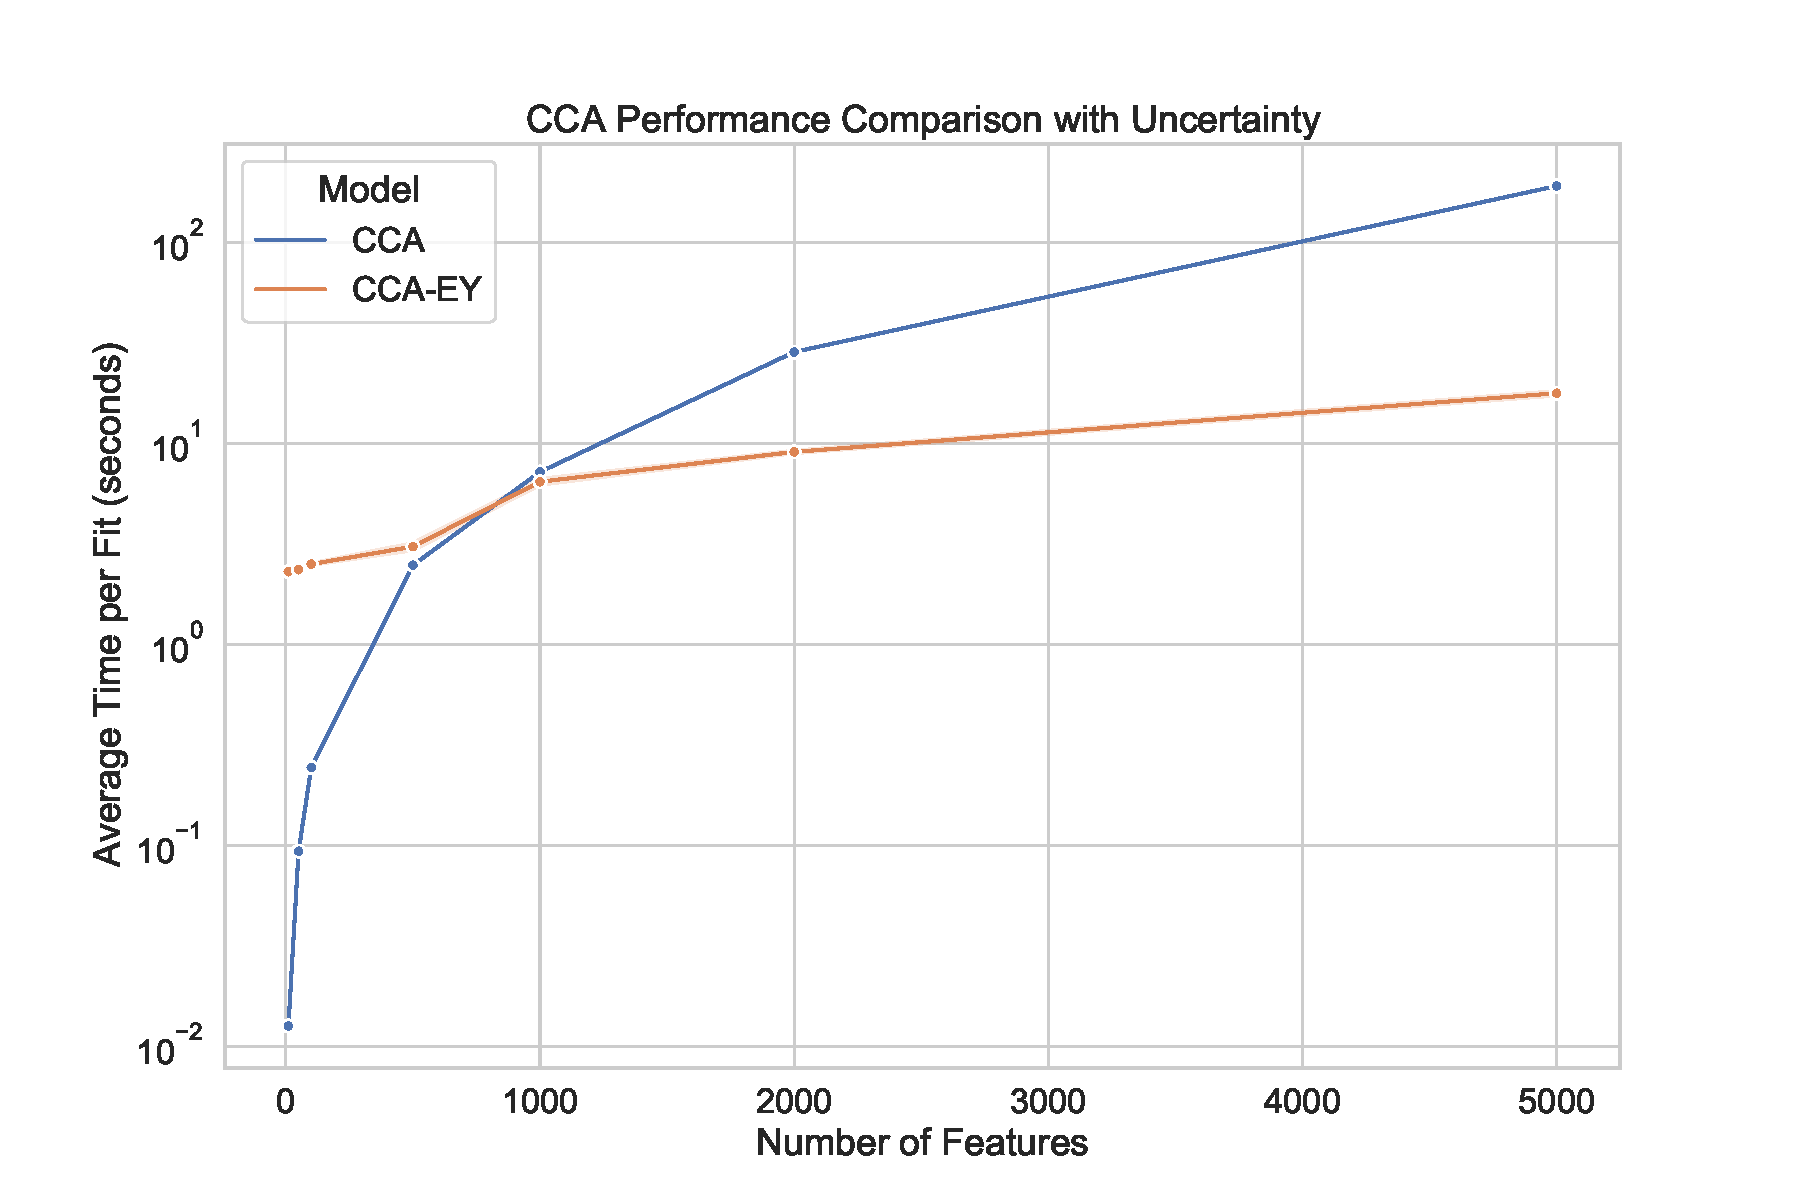
\includegraphics[width=0.8\textwidth]{figures/benchmarks/cca_comparison_log}
    \caption{Comparison of the time taken to solve CCA using \texttt{eigh} and our CCA-EY method.}
    \label{fig:cca-comparison}
\end{figure}

\subsection{Stochastic CCA on Real-World Datasets}
In this experiment, we evaluate the performance of our proposed CCA-EY method against two established baselines, $\gamma$-EigenGame \citep{gemp2022generalized} and SGHA \citep{chen2019constrained}, on real-world datasets. Our experimental setup follows the framework introduced by \citet{meng2021online} and \citet{gemp2022generalized}, with a key difference: we do not perform PCA on the data prior to applying the CCA methods. This choice allows us to assess the algorithms' ability to handle high-dimensional data efficiently and accurately, without the aid of dimensionality reduction.
\subsubsection{Data}
We use two datasets for this experiment:

MediaMill \citep{gemert2008visual}: This dataset consists of paired features extracted from videos and their corresponding textual commentary. The goal is to learn joint representations that capture the correlation between the visual and textual modalities. The dataset includes 25,800 test instances, with 120 and 101 features for the video and commentary views, respectively.
Split-CIFAR \citep{meng2021online}: This dataset is derived from the CIFAR-10 image classification dataset. Each RGB image is split in half, resulting in two views with 32x16x3 features each. The objective is to learn joint representations of the two halves that reveal correlations, which are expected to be high within the same class and low across different classes. The dataset contains 50,000 training and 10,000 test instances.

These datasets were chosen for their diverse nature and complexity, providing a comprehensive test bed for evaluating the performance of stochastic CCA methods.
\subsubsection{Experimental Setup and Evaluation Metric}
We train the CCA models on the MediaMill and Split-CIFAR datasets for a single epoch, using mini-batch sizes ranging from 5 to 100. These batch sizes were selected to assess the scalability and efficiency of the methods under varying computational loads.
To evaluate the performance of the algorithms, we use the Proportion of Correlation Captured (PCC) metric, defined as:
\begin{equation}
\text{PCC} = \frac{\sum_{k=1}^K \rho_k}{\sum_{k=1}^K \rho_k^*},
\end{equation}
where $K$ is the number of canonical components, $\rho_k$ represents the correlations of the estimated representations $Z\sps{i}=X^{(i)}\hat{U}^{(i)}$ with one another on the test set, while $\rho_k^*$ denotes the canonical correlations computed from the full batch covariance matrices.
In other words, using our earlier notation, $\rho_k = \MCCA_K(\hat{Z}\sps{1}, \hat{Z}\sps{2})$ and $\rho_k^* = \MCCA_K(X\sps{1}, X\sps{2})$.
Although $\rho_k^*$ are not strictly the ground-truth correlations, they serve as a reliable benchmark when computed from a large sample size. The PCC metric provides an efficient way to track the performance of the algorithms over time while minimizing computational overhead \citep{meng2021online, gemp2022generalized, ma2015finding, ge2016efficient}.
For each method, we perform a grid search over the hyperparameters listed in Table \ref{tab:hyperparameters} using the Weights and Biases platform \citep{wandb}.
\begin{table}[h!]
    \centering
    \begin{tabular}{|l|l|}
        \hline Parameter             & Values              \\
        \hline minibatch size        & 5,20,50,100         \\
        \hline components            & 5                   \\
        \hline epochs                & 1                   \\
        \hline seed                  & 1, 2, 3, 4, 5       \\
        \hline lr                    & 0.01, 0.001, 0.0001 \\
        \hline $\gamma$\footnote{gamma is only used for $\gamma$-EigenGame} & 0.01,0.1,1,10       \\
        \hline
    \end{tabular}
    \caption{Hyperparameter ranges explored for CCA methods.} 
    \label{tab:hyperparameters}
\end{table}
\subsubsection{Results and Observations}
Figure \ref{fig:corr_mediamill} compares the learning curves of the algorithms on the MediaMill dataset for various mini-batch sizes. CCA-EY consistently outperforms the baselines across all batch sizes. Figure \ref{fig:learningcurve_mediamill} provides a more detailed view of the learning curves for batch sizes 5 and 100, highlighting the superior performance of CCA-EY over time.
\begin{figure}
\centering
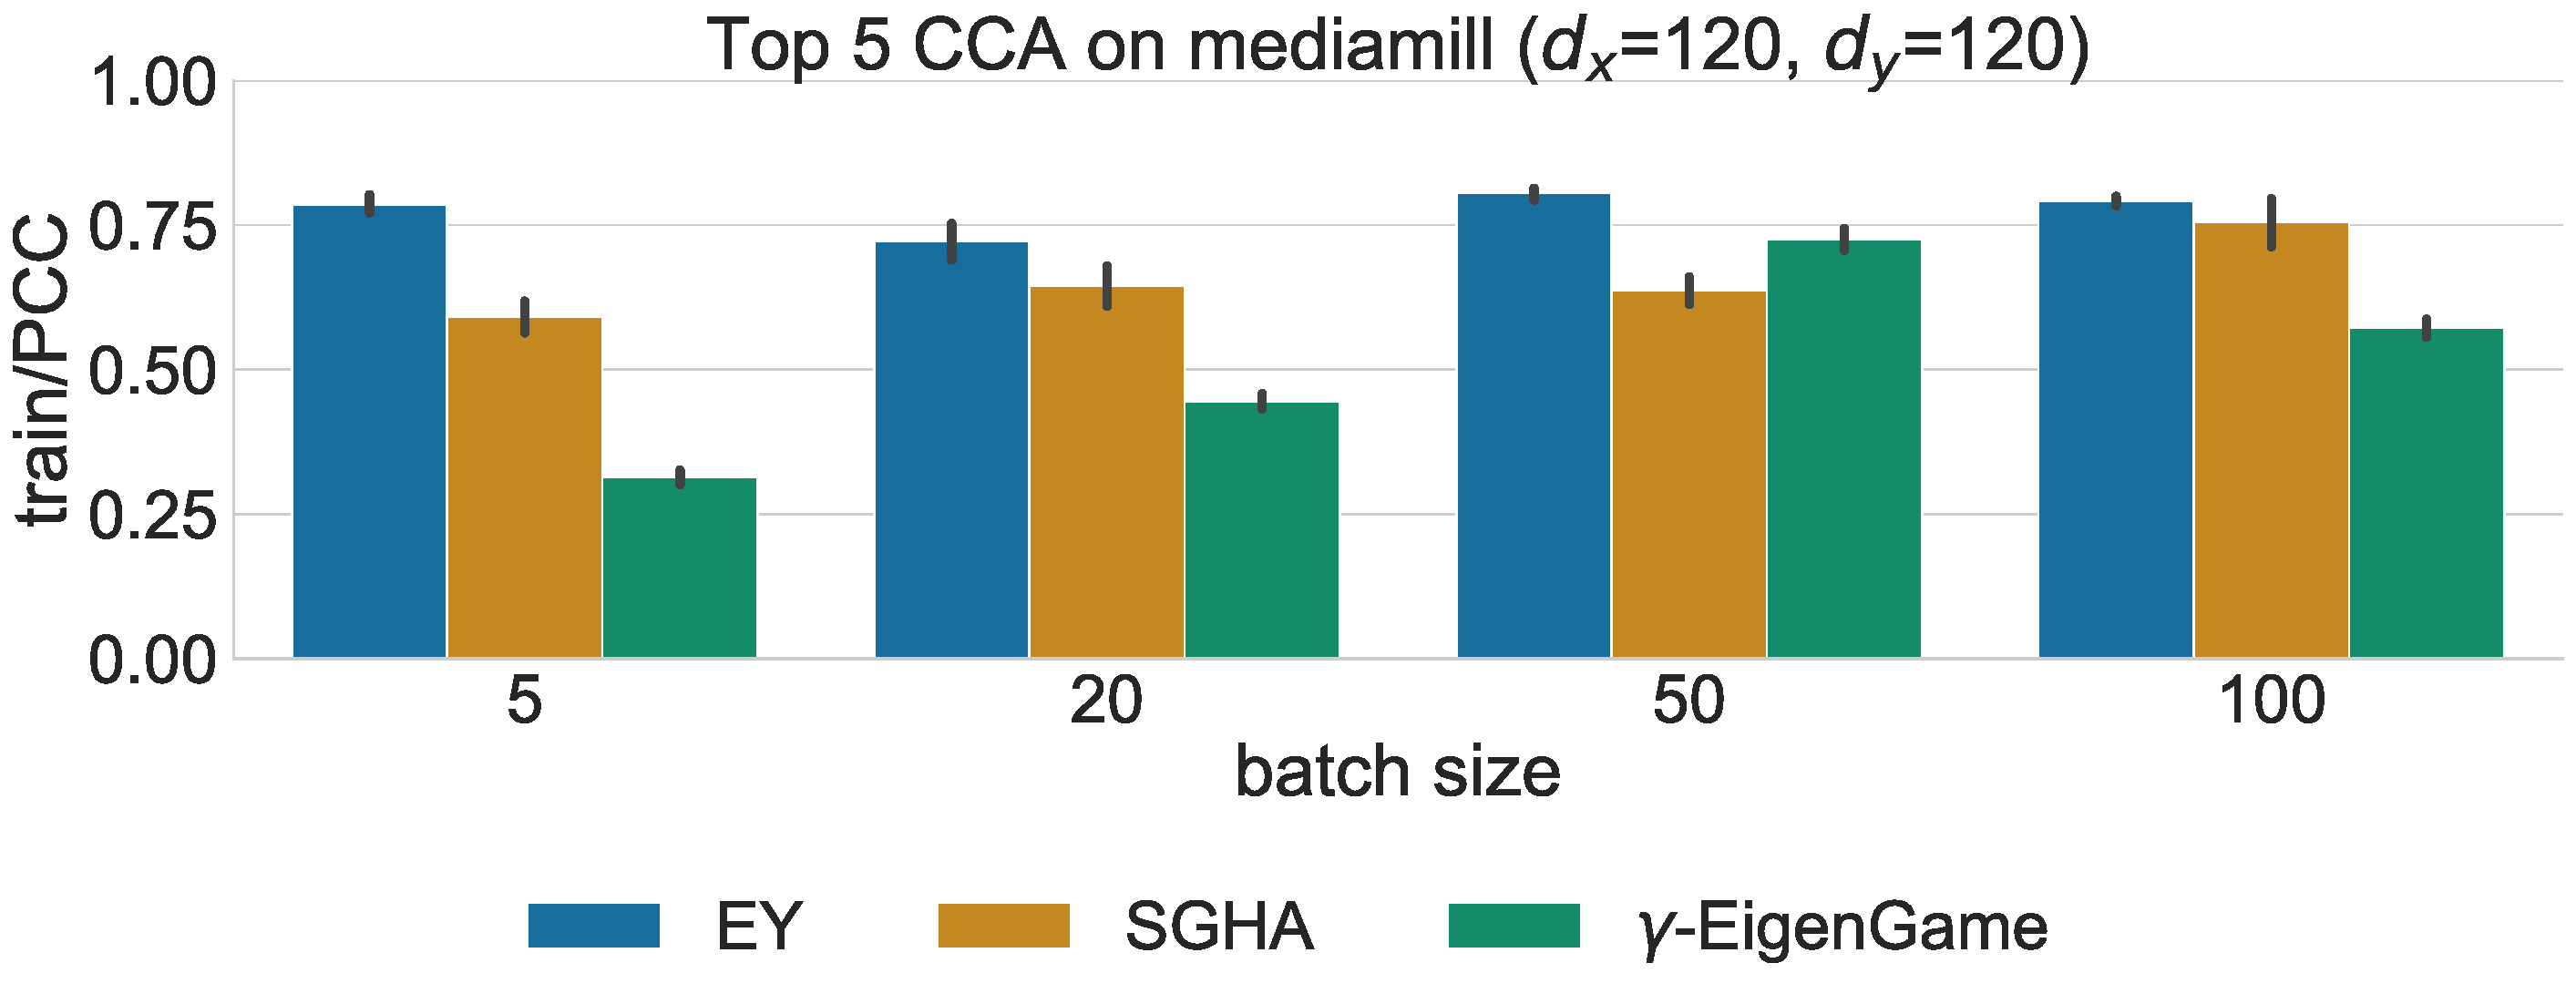
\includegraphics[width=0.8\textwidth]{figures/CCA/mediamill_models_different_batch_sizes}
\caption{Stochastic CCA on MediaMill using PCC: Performance across varying mini-batch sizes. Shaded regions represent $\pm$ one standard deviation around the mean of 5 runs.}
\label{fig:corr_mediamill}
\end{figure}
\begin{figure}
\centering
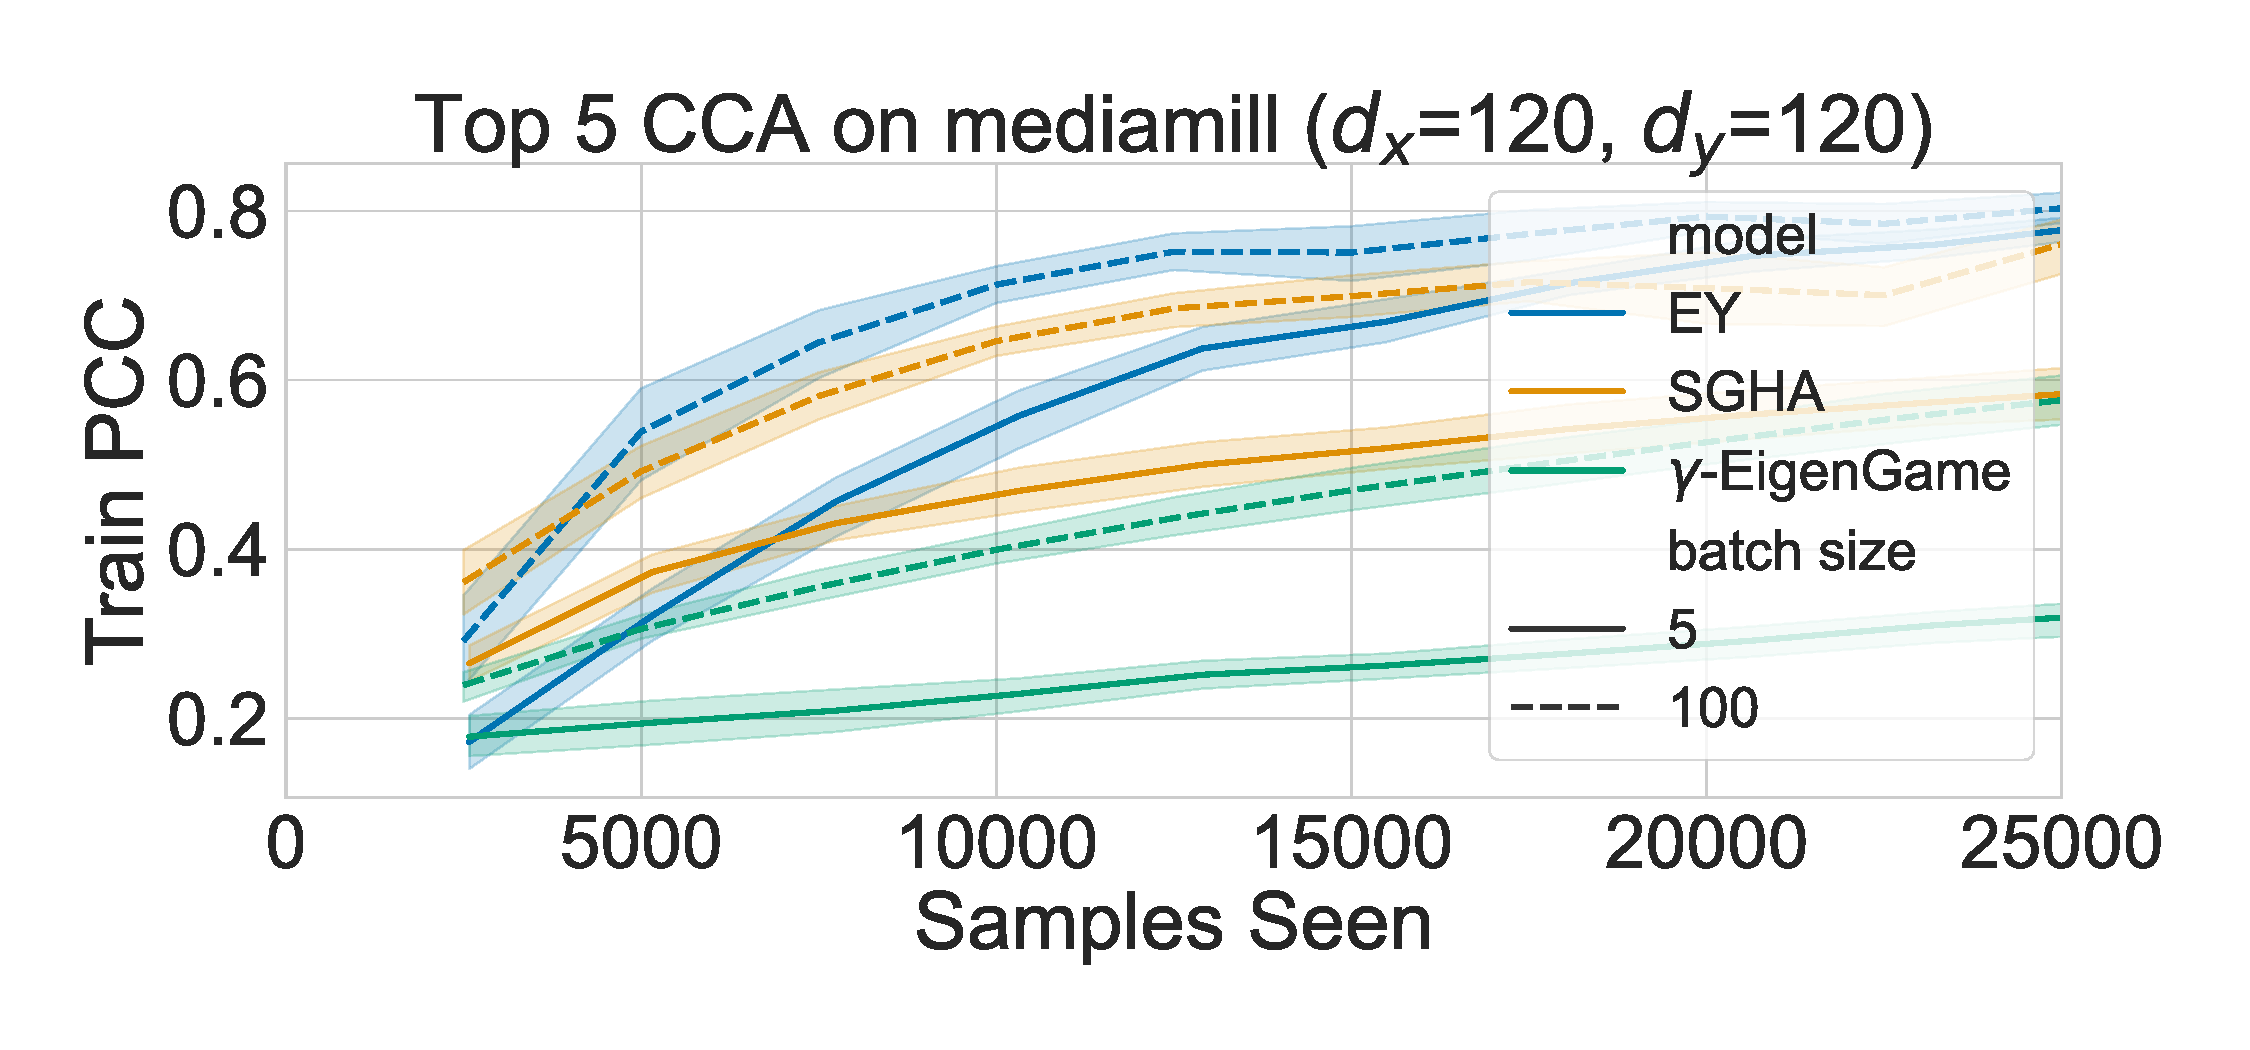
\includegraphics[width=0.8\textwidth]{figures/CCA/mediamill_allbatchsizes_pcc}
\caption{Stochastic CCA on MediaMill: Training progress over a single epoch for mini-batch sizes 5 and 100.}
\label{fig:learningcurve_mediamill}
\end{figure}
For the Split-CIFAR dataset, Figure \ref{fig:corr_cifar} shows the performance comparison across batch sizes, while Figure \ref{fig:learningcurve_cifar} presents the learning curves. The results reveal that $\gamma$-EigenGame underperforms compared to CCA-EY and SGHA, particularly for smaller batch sizes.
\begin{figure}
\centering
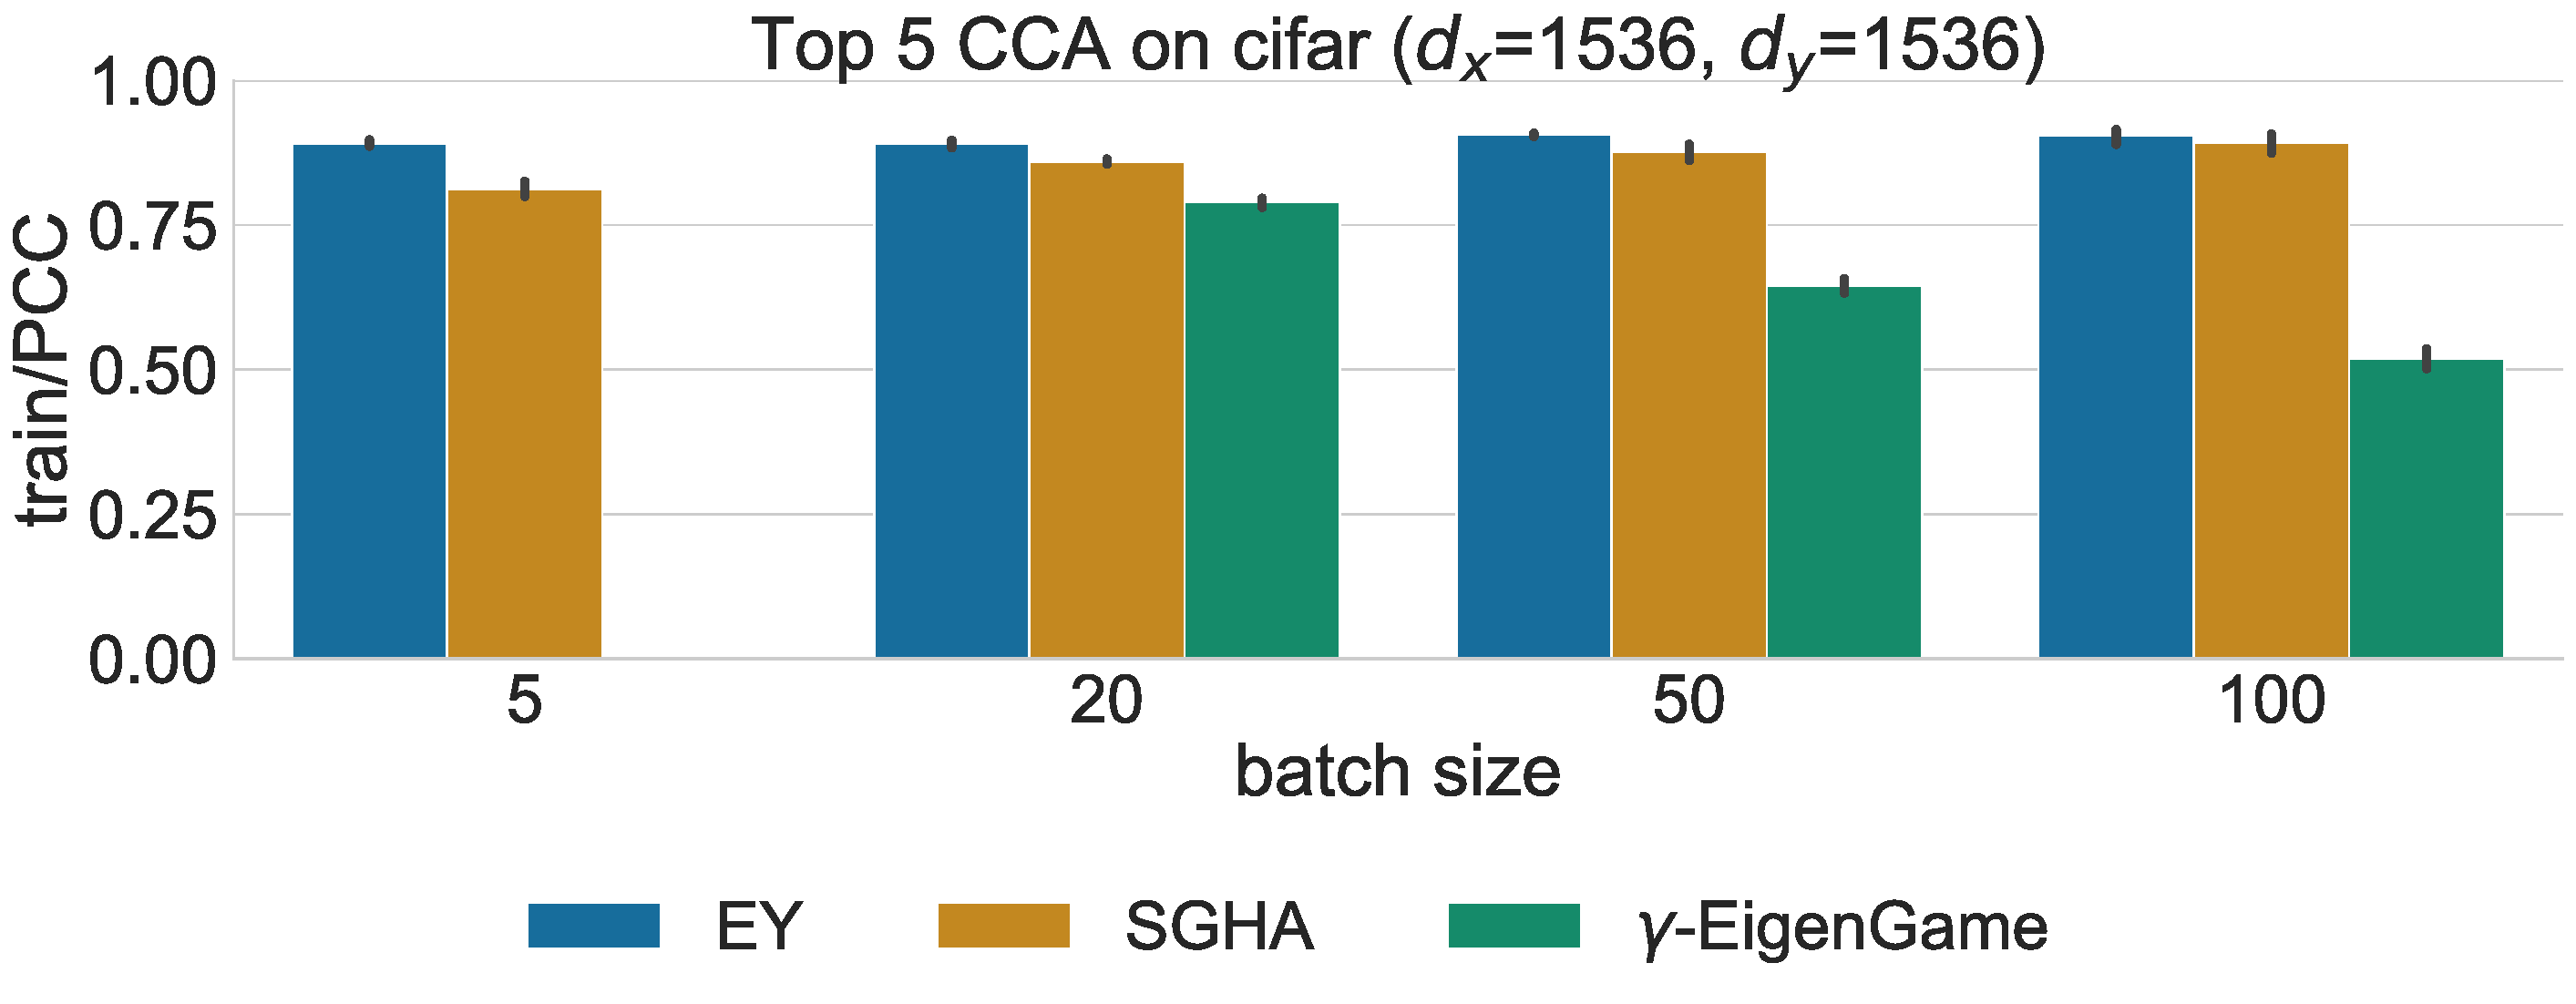
\includegraphics[width=0.8\textwidth]{figures/CCA/cifar_models_different_batch_sizes}
\caption{Stochastic CCA on Split-CIFAR using PCC: Performance across varying mini-batch sizes. Shaded regions represent $\pm$ one standard deviation around the mean of 5 runs.}
\label{fig:corr_cifar}
\end{figure}
\begin{figure}
\centering
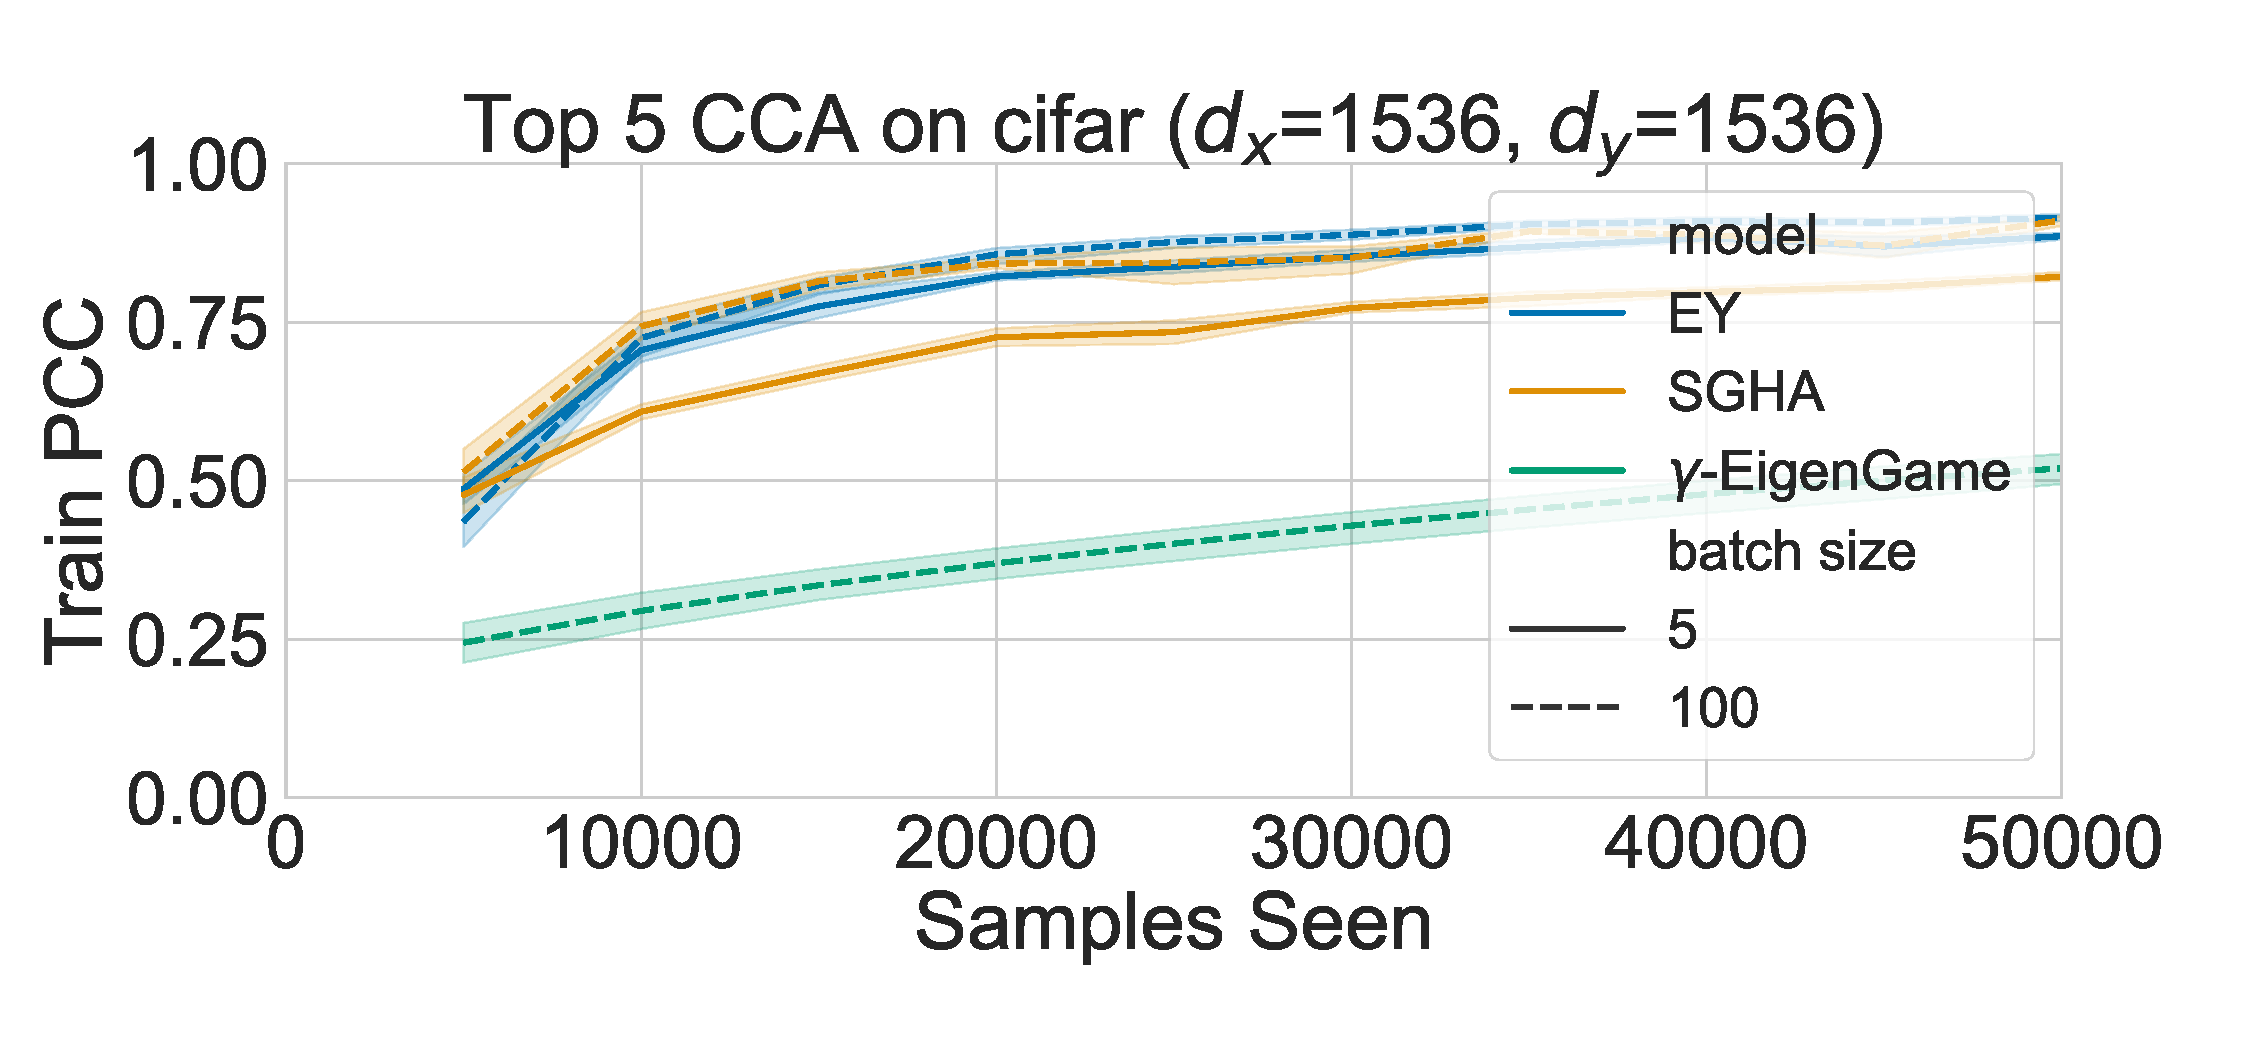
\includegraphics[width=0.8\textwidth]{figures/CCA/cifar_allbatchsizes_pcc}
\caption{Stochastic CCA on Split-CIFAR: Training progress over a single epoch for mini-batch sizes 5 and 100.}
\label{fig:learningcurve_cifar}
\end{figure}
These experiments demonstrate that our proposed CCA-EY method can achieve faster convergence with less hyperparameter tuning compared to the established baselines, making it a promising approach for practical applications involving high-dimensional data.

\subsection{Stochastic PLS on UK Biobank Data}
In this experiment, we showcase the scalability and efficiency of our Stochastic PLS method, PLS-EY, on an extremely high-dimensional imaging genetics dataset from the UK Biobank \citep{sudlow2015uk}.
\subsubsection{Data}
The UK Biobank is a large-scale biomedical database containing genetic and phenotypic data from over 500,000 participants. For this experiment, we use a subset of the data consisting of brain imaging features (82 regional volumes) and genetic variants (582,565 SNPs) for 33,333 subjects.
The brain imaging data was preprocessed using FreeSurfer \citep{Fischl2012} to extract gray-matter volumes for 66 cortical regions (based on the Desikan-Killiany atlas) and 16 subcortical regions. The effects of age, age squared, intracranial volume, sex, and the first 20 genetic principal components (to account for population structure) were regressed out from the brain features. Each brain region of interest (ROI) was then normalized by removing the mean and dividing by the standard deviation.
The genetic data was processed using PLINK \citep{Purcell2007}, retaining genetic variants with a minor allele frequency of at least 1% and a maximum missingness rate of 2%. Mean imputation was used to fill in missing values, and each variant was centered.
To generate measures of genetic disease risk, we calculated polygenic risk scores using PRSice \citep{PRSice2014}. Scores were computed with a p-value threshold of 0.05 using GWAS summary statistics for the following diseases: Alzheimer's \citep{Lambert2013}, Schizophrenia \citep{Trubetskoy2022}, Bipolar disorder \citep{Mullins2021}, ADHD \citep{Demontis2023}, ALS \citep{Van_Rheenen2021}, Parkinson's disease \citep{Nalls2019}, and Epilepsy \citep{International_League_Against_Epilepsy_Consortium_on_Complex_Epilepsies2018}.
\subsubsection{Experimental Setup}
We apply our PLS-EY method to the UK Biobank dataset, using a mini-batch size of 500 and training for 100 epochs with a learning rate of 0.0001. A key computational challenge in this experiment is maintaining orthogonality between the weight vectors $u_k$ in the PLS model, which is crucial for the method's effectiveness.
This approach allows us to handle the high-dimensional nature of the data while preserving the interpretability of the learned representations. To the best of our knowledge, this experiment represents the largest-scale PLS analysis of biomedical data to date, demonstrating the potential of our method to facilitate discoveries in extremely large datasets.
\subsubsection{Results and Observations}
Figure \ref{fig:UKBB_corr} shows the Pearson correlations among the PLS latent variables $Z_k$ derived from the UK Biobank data. We observe strong correlations between corresponding pairs of representations $Z^{(1)}_k$ and $Z^{(2)}_k$, and weak cross-correlations between $Z^{(1)}_k$ and $Z^{(2)}_i$ for $i \neq k$. This indicates that our PLS-EY model learns a coherent and orthogonal subspace.
\begin{figure}
\centering
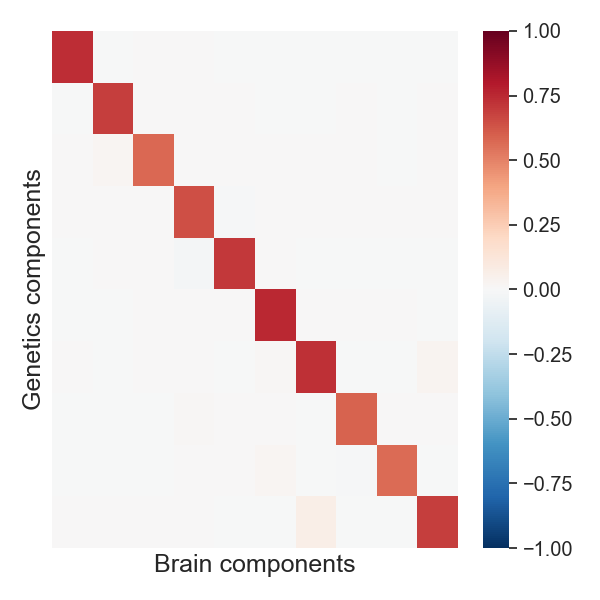
\includegraphics[width=0.6\textwidth,trim={0.8cm 0cm 0.3cm 0cm}]{figures/UKBB/cross_corr.png}
\caption{Pearson correlations among PLS latent variables $Z_k$ derived from UK Biobank data.}
\label{fig:UKBB_corr}
\end{figure}
Furthermore, we investigate the associations between the PLS brain representations $Z$ and the polygenic risk scores for various disorders, as shown in Figure \ref{fig:genetic_risk}. The results reveal significant correlations between the learned representations and genetic risk measures for several disorders, suggesting that the PLS subspace captures relevant information for genetic disease risk. This finding has important implications for biomedical research, as it demonstrates the ability of our method to uncover meaningful relationships in high-dimensional data.
\begin{figure}
\centering
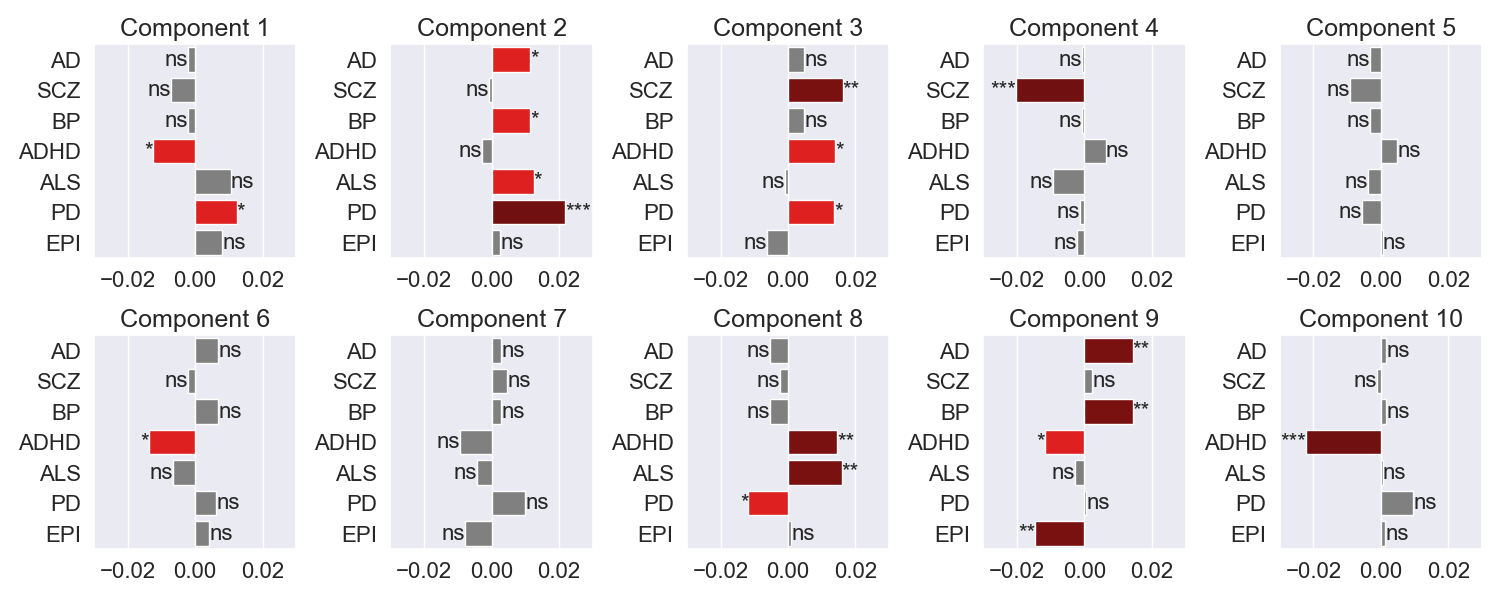
\includegraphics[width=0.99\textwidth,trim={0.5cm 0cm 0.7cm 0cm}]{figures/UKBB/prs_correlations.png}
\caption{Correlation between PLS brain representations $Z$ and genetic risk scores for various disorders. AD=Alzheimer's disease, SCZ=Schizophrenia, BP=Bipolar disorder, ADHD=Attention deficit hyperactivity disorder, ALS=Amyotrophic lateral sclerosis, PD=Parkinson's disease, EPI=Epilepsy. $\text{ns}: 0.05 < p \leq 1, \ast: 0.01 < p \leq 0.05, \ast\ast: 0.001 < p \leq 0.01, \ast\ast\ast: 0.0001 < p \leq 0.001$.}
\label{fig:genetic_risk}
\end{figure}
These results demonstrate the scalability of our PLS-EY method to extremely high-dimensional data and its ability to learn interpretable representations that capture biologically relevant information. The successful application of our method to the UK Biobank dataset highlights its potential to facilitate discoveries in large-scale biomedical studies.

\section{Discussion}

\subsection{Limitations}

This chapter presents a comprehensive exploration and development of novel algorithms for Canonical Correlation Analysis (CCA) and Partial Least Squares (PLS), focusing on scalability and efficiency in high-dimensional and large-scale datasets.
Our approach introduces the Eckhart-Young (EY) inspired objectives for Generalized Eigenvalue Problems (GEPs) and their application in stochastic or data-streaming settings, paving the way for more efficient and scalable solutions to classical subspace learning problems.

Our proposed CCA-EY and PLS-EY methods demonstrate significant advancements over traditional approaches in handling the computational complexity and scalability issues inherent in high-dimensional data.
By reformulating the CCA and PLS objectives, we provide a path to efficiently analyze large datasets, which was previously infeasible due to computational limitations.
The empirical evaluation on diverse datasets, including MediaMill, Split-CIFAR-10, and the UK Biobank, not only validates the effectiveness of our methods but also highlights their superiority in convergence speed and robustness to hyperparameter tuning.

The results from the MediaMill and Split-CIFAR-10 datasets underscore the potential of CCA-EY in achieving faster convergence with minimal hyperparameter tuning, a crucial factor for practical applications.
This advantage is particularly pronounced when comparing our method to established baselines like $\gamma$-EigenGame and SGHA. Additionally, the application of our methods to the UK Biobank dataset represents a breakthrough in the analysis of imaging genetics data, showcasing the capability of PLS-EY to manage extraordinarily high-dimensional data while extracting meaningful and interpretable representations.

Furthermore, our methods' ability to capture relevant information for genetic disease risk, as evidenced in the UK Biobank study, opens new avenues for biomedical research.
The significant associations between the PLS representations and genetic risk measures for various disorders provide valuable insights into the genetic mechanisms underlying diseases and brain morphometry.

\subsection{Future Work}

\subsection{Proximal Gradient Descent for Regularized GEPs}

Our future initiatives will enhance CCA, PCA and PLS by incorporating proximal gradient descent for efficient handling of complex regularization terms. This methodology is ideally suited for scenarios where the loss function comprises a smooth, differentiable component plus a non-smooth regularization term. The proximal gradient technique uses a gradient step followed by a proximal step, enabling effective management of non-smooth penalties such as L1-norm or Total Variation (TV), which are instrumental in enforcing sparsity and structural constraints.

\subsubsection{Objective Formulation with Regularization}

We aim to modify the CCA framework by integrating specific regularization terms directly into the loss function of the Generalized Eigenvalue Problem (GEP). The revised loss function, denoted as $\mathcal{L}_{\text{Proximal CCA-EY}}(\mathbf{U}_1, \mathbf{U}_2)$, will incorporate the regularization terms $R_1(\mathbf{U}_1)$ and $R_2(\mathbf{U}_2)$, enabling the optimization of CCA with additional constraints. The objective function for Proximal CCA-EY will be defined as:

\begin{align*}
    \mathcal{L}_{\text{Proximal CCA-EY}}(\mathbf{U}_1, \mathbf{U}_2) &= \mathcal{L}_{\text{EY}}(\mathbf{U}_1, \mathbf{U}_2)
    + \lambda_1 R_1(\mathbf{U}_1) + \lambda_2 R_2(\mathbf{U}_2),
\end{align*}

where $\mathcal{L}^{\text{Proximal CCA-EY}}$ represents the Proximal CCA-EY loss function, $\lambda_1$ and $\lambda_2$ are regularization parameters, and $R_1(\mathbf{U}_1)$ and $R_2(\mathbf{U}_2)$ are the regularization terms for each view.

\subsubsection{Proximal Gradient Descent Mechanism}

The proximal gradient updates for this augmented CCA formulation are specified as:

\begin{align}
\mathbf{U}1^{(t+1)} &= \text{prox}{\alpha \lambda_1 R_1}(\mathbf{U}_1^{(t)} - \alpha \nabla{\mathbf{U}_1} \mathcal{L}^{\text{EY}}(\mathbf{U}_1^{(t)}, \mathbf{U}_2^{(t)})), \
\mathbf{U}2^{(t+1)} &= \text{prox}{\alpha \lambda_2 R_2}(\mathbf{U}_2^{(t)} - \alpha \nabla{\mathbf{U}_2} \mathcal{L}^{\text{EY}}(\mathbf{U}_1^{(t)}, \mathbf{U}_2^{(t)})),
\end{align}

where $\text{prox}_{\alpha \lambda_i R_i}(\mathbf{v})$ denotes the proximal operator for the regularization term $R_i$ with parameter $\lambda_i$, and $\alpha$ represents the learning rate. Note that the gradients $\nabla{\mathbf{U}_1} \mathcal{L}^{\text{EY}}(\mathbf{U}_1^{(t)}, \mathbf{U}_2^{(t)})$ and $\nabla{\mathbf{U}_2} \mathcal{L}^{\text{EY}}(\mathbf{U}_1^{(t)}, \mathbf{U}_2^{(t)})$ are computed only for the smooth part of the loss function, i.e., $\mathcal{L}^{\text{EY}}(\mathbf{U}_1, \mathbf{U}_2)$, and do not include the regularization terms.

The proximal operator is defined as solving:

\begin{align*}
\text{prox}{\alpha \lambda_i R_i}(\mathbf{v}) = \arg \min\mathbf{u} \left( R_i(\mathbf{u}) + \frac{1}{2\alpha} |\mathbf{u} - \mathbf{v}|_2^2 \right).
\end{align*}

This update effectively balances the influence of the gradient of the smooth loss function and the geometry imposed by the regularization, making the approach robust to the inclusion of complex constraints in the optimization of CCA.

\subsubsection{Efficiency and Applicability}

The proximal gradient descent method excels in large-scale optimization challenges where traditional techniques struggle due to the presence of non-smooth terms. By separating the optimization of the smooth component from the non-smooth regularization, proximal steps can be efficiently computed, particularly when $R_i$ allows a straightforward proximal formulation.

\subsection{Conclusion}

In summary, this chapter contributes to the fields of machine learning and multiview data analysis by introducing scalable and efficient solutions for CCA and PLS, applicable in a variety of domains, including but not limited to neuroimaging and genetics.
Our work not only addresses significant computational challenges but also lays the groundwork for future research and practical applications in analyzing large-scale, high-dimensional datasets.